\documentclass[tikz]{standalone}

\usetikzlibrary{arrows}
\usetikzlibrary{arrows.meta}

\begin{document}

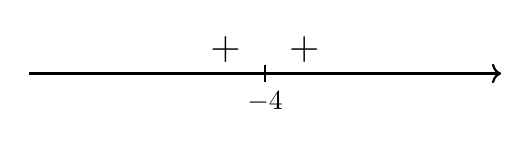
\begin{tikzpicture}[baseline=-0.5ex,scale=0.5]
    \draw[thick,->] (-10,0) -- (2,0);
    
    \node at (-5,0.6) {\Large $+$};
    \node at (-3,0.6) {\Large $+$};
    
    \foreach \x in {-4} 
        \draw [thick] (\x cm,6pt) -- (\x cm,-6pt) node[below] {$\x$};
\end{tikzpicture}

\begin{tikzpicture}[baseline=-0.5ex,scale=0.5]
    \draw[thick,->] (-10,0) -- (2,0);
    
    \node at (-5,0.6) {\Large $+$};
    \node at (-3,0.6) {\Large $-$};
    
    \foreach \x in {-4} 
        \draw [thick] (\x cm,6pt) -- (\x cm,-6pt) node[below] {$\x$};
\end{tikzpicture}



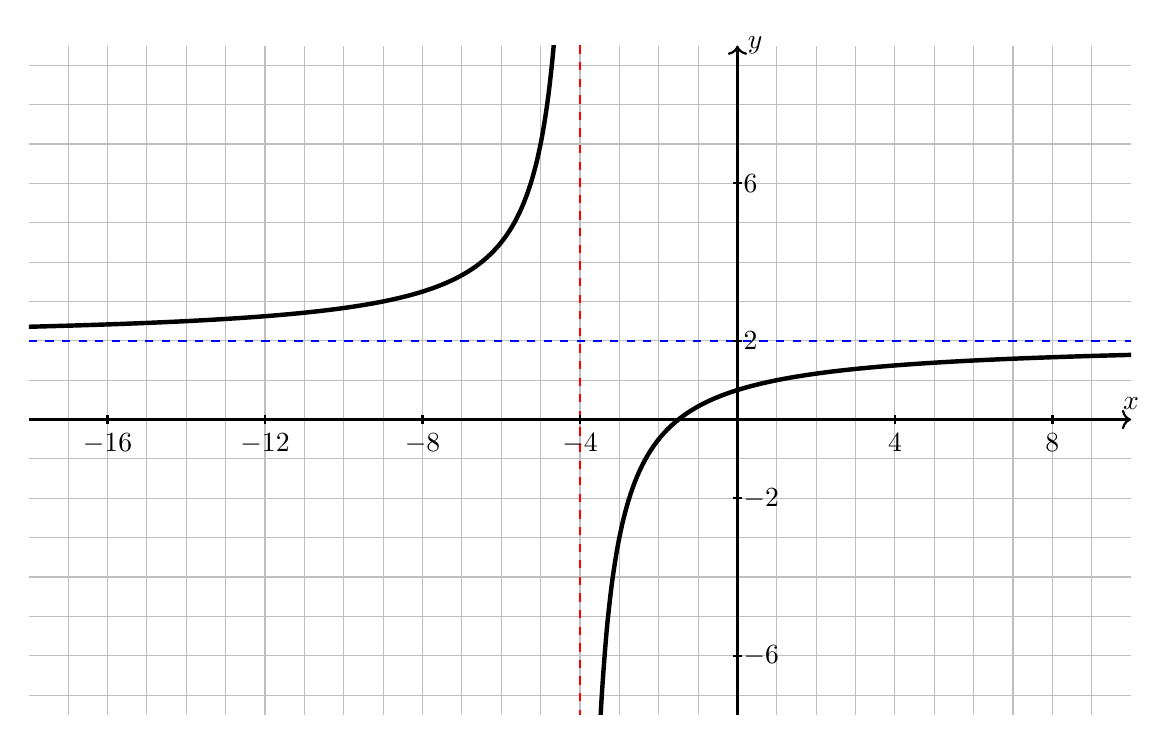
\begin{tikzpicture}[ultra thick,smooth,domain=-6:6,variable=\x,scale=0.5]

    % create a white background with a black frame
    % \draw [thin,fill=white] (-19,-8.5) rectangle (11,10.5);  
    
    % draw grid
    \draw[xstep=1.0cm, ystep=1.0cm, lightgray, thin] (-17.99,-7.5) grid (9.99,9.5); 
    
    % draw axes
    \draw [->,thick] (-18,0) -- (10,0) node[above] {$x$};
    \draw [->,thick] (0,-7.5) -- (0,9.5) node[right] {$y$};
    
    
    \clip (-18,-7.5) rectangle (10,9.5);
    
    % (2x+3) / (x+4)
    \draw plot [domain=-18:-4.1,samples=100] (\x,{(2*\x + 3) / (\x + 4)}); 
    \draw plot [domain=-3.9:10,samples=100] (\x,{(2*\x + 3) / (\x + 4)}); 
    
    % asymptotes
    \draw[dashed,red,thick] (-4,-8) -- (-4,10);
    \draw[dashed,blue,thick] (-18,2) -- (10,2);
    
    % tick marks
    \foreach \x in {-16,-12,-8,-4,4,8} 
        \draw [thick] (\x cm,3pt) -- (\x cm,-3pt) node[below] {$\x$};
    \foreach \y in {-6,-2,2,6} 
        \draw [thick] (3pt,\y cm) -- (-3pt,\y cm) node[right] {$\y$};
\end{tikzpicture}

\end{document} 